%----------------------------------------------------------------------------------------
%	CHAPTER 3
%----------------------------------------------------------------------------------------

\chapterimage{boat.png}
\chapter{Understand your data}

Before continuing, first and most importantly you must select the \emph{raw} data you are going to process and later after you acquire experience with an specific dataset the idea is to expand the algorithms to any kind of dataset. The important things are to learn how to input the data correctly, establish the right \emph{learning parameters} in the selected algorithm and find the best way to visualize your results and interpret them correctly.

Now let's start with basic concepts that vary from an engineering to an astronomer point of view.
\section{What is an image?}
	As you may know, an image is a matrix of numbers that contains the specific brightness level that corresponds to a given pixel. And from there the concepts evolves and adds channels of colour and depth. But for now, let's just think about monochromatic images (only one channel). In Astronomy, images are usually considered sets of scientific data, observations, that contain information about an specific target in the sky seen through an specific filter and the levels of brightness correspond to the behaviour of the optical sensor (CCD camera) in relation with the number of electrons that hit a particular pixel through an specific waveband. Something else to consider is that the sky is not flat with this I mean that the celestial vault is like a sphere surrounding us therefore Cartesian coordinates are not the parameters used to identify points in space, there is another system called WCS (World Coordinate System) hence a conversion between pixels and WCS coordinates exists. As you are realizing now just one image can contain tons of information related to it, now imagine that multiplied for terabytes and terabytes of stars, galaxies, planets, nebulae or any object in space. Fortunately in astronomy this is solved using an image format that contains the image and its own information.
	\subsection{FITS files}
    	This format is the standard data format used in astronomy, can contain one image, multiple images, tables and header keywords providing descriptive information about the data. The way it works is that this format can contain a text file with keywords that comprise the information about the observation and a multidimensional array that could be a table, or an image, or an array of images (data cube). This files can be managed in different ways, with an image preview use DS9, for handing the data in a program use the \emph{Python} package \emph{PyFITS}.
        
	\subsection{WFC3 ERS M83 Data Products}
    The selected dataset to test the data mining libraries I found is a series of observations of M83 at 9 different wavelengths, the original images can be found in this web page, \url{http://archive.stsci.edu/prepds/wfc3ers/m83datalist.html}, the specific information about them can be found in Table \ref{tab:uno}. This particular images were observed through HST with the WFC3/UVIS camera.
    
\begin{table}[h]
  \centering
  \begin{tabular}{ c c c c c c }
    \hline\hline
    Filter / Config. & Waveband / Central $\lambda$/ Line & Obs. Date & Comment \\
    \hline
    F225W & UV filter / 235.9 nm & 26 Aug 2009 &  UV wide\\
    
    F336W & UV filter / 335.5 nm & 26 Aug 2009 & Str$\ddot{o}$mgren $u$\\
    
    F373N & Narrow-Band Filter / 373.0 nm & 19 Aug 2009 & Includes \textsc{[OII]}\\
    
    F438W & Wide-Band Filter / 432.5 nm & 26 Aug 2009 & $B$, Johnson-Cousins set\\
    
    F487N & Narrow-Band Filter / 487.1 nm & 25 Aug 2009 & Includes H$\beta$\\
    
    F502N & Narrow-Band Filter / 501.0 nm & 26 Aug 2009 & Includes \textsc{[O III]}\\
    
    F657N & Narrow-Band Filter / 656.7 nm & 25 Aug 2009 & Includes H$\alpha$+\textsc{[NII]}\\
    
    F673N & Narrow-Band Filter / 676.6 nm & 20 Aug 2009 & Includes \textsc{[SII]}\\
    
    F814W & Wide-Band Filter / 802.4 nm & 26 Aug 2009 & $I$, Johnson-Cousins set\\
    \hline
  \end{tabular}
  \caption{Summary of Observations}
  \label{tab:uno}
\end{table}
%Poner aqui la tabla con los datos de acada filtro
%No olvidar poner en GitHub el programa de como hacer el cube y tammbien el de reproject cube con montrage wrapper

\section{Preprocessing your data}
This section is where you prepare your data to be processed, you have to make sure that all your images have the same grid size, same spatial resolution, less possible quantity of outliers and noise and same coordinate system. Now, what are those things? Same grid size means that your images must have the same pixel size, in the dataset we are processing we don't have to worry about this, the pixel size is 0.0396 arc sec/pixel. Now, spatial resolution, each image has it's own spatial resolution depending on the filter that was used to get the observation, the number that you will be looking for is the FWHM that describes the PSF of every image. When you have all the FWHM for all the images you should choose the largest which corresponds to the poorest spatial resolution and create a convolution kernel with \emph{Tiny Tim} or use a Gaussian kernel calculated with \emph{Astropy} and convolve all the images with that kernel. This exactly what I did, if you look at image \ref{mg:conv}, you will see the before and after convolution. In table \ref{tab:dos} you can see how I chose the number for the FWHM.

\begin{figure}[h]
	\centering
    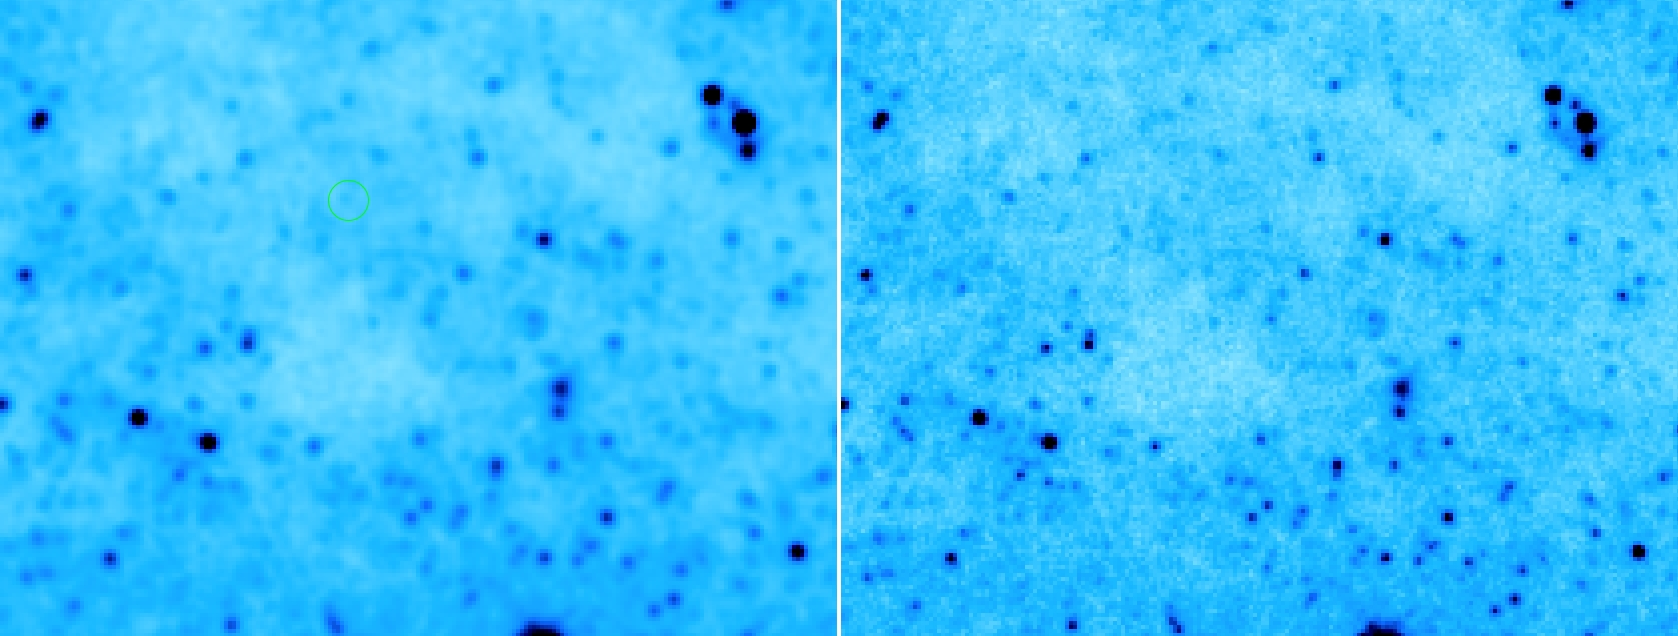
\includegraphics[width=0.87\textwidth]{conv.jpg}
    \caption{In this image you can observe how an observation looks, before and after convolution, this particular image corresponds to the B band filter and was convolved to a 0.083 arc sec FWHM}
    \label{img:conv}
\end{figure}

\begin{table}[h]
  \centering
    \begin{tabular}{ c c c }
    \hline\hline
    
    Filter / Config. & Central $\lambda$ & FWHM (arc sec)\\
    \hline
    
    F225W & 235.9 nm & $\sim$0.083\\
    
    F336W & 335.5 nm & $\sim$0.075\\
    
    F373N & 373.0 nm & $\sim$0.070\\
    
    F438W & 432.5 nm & $\sim$0.070\\
    
    F487N & 487.1 nm & $\sim$0.067\\
    
    F502N & 501.0 nm & $\sim$0.067\\
    
    F657N & 656.7 nm & $\sim$0.070\\
    
    F673N & 676.6 nm & $\sim$0.070\\
    
    F814W & 802.4 nm & $\sim$0.074\\
    
    \hline
  \end{tabular}
  \caption{WFC3/UVIS PSF FWHM informations for the selected dataset, as you can see the largest number here is 0.083 which means the poorest spatial resolution, this is the number used to calculate the convolution kernel, in order to precess them all images must have the same spatial resolution.}
  \label{tab:dos}
\end{table}

After convolving all the pictures, I started to do some tests, but I realized that maybe around 30\% of the images was missing information and/or noise and the results I was getting were mislead by the outliers. In clustering algorithms we must help the algorithm, make sure that what we are inputting is something that can be clustered, although some of them are \emph{shielded} against outliers, making our data more accessible and easy for the neural networks to interpret will help you to get better results, as you can see in image \ref{img:dos} (open one and explore it in DS9) there is missing information and noise. In order to correct this I decided to go with the easiest way I could think of, just cut the image. And I did selected a processable area excluding all the missing information and noisy areas.

\begin{figure}[h]
	\centering
    \includegraphics[width=0.47\textwidth]{uno.jpg}
    \caption{Look at the image, it is composed of two mosaics, therefore, there are some regions with missing data, now look at the borders of each mosaic there is noise near the edges, this is data that we don't want messing with our clustering algorithm and can be classified as outliers, it is very important to reduce them as much as possible so the output clusters can be correctly classified and correspond to the information that we are looking for}
    \label{img:dos}
\end{figure}

The next step was to build the data cube, at this point you can decide if you want to process your images independently or all of them. The ideal here is to input all of them in a data cube, so the output clusters relate information from all the wavelengths and the regions covered by them can be interpreted more easily. Now if you choose to create an image cube (just append the image arrays in one FITS file) it is possible that your images have a different conversion between their world coordinate system to pixel, so have to make sure all of your images are projected with only one conversion, this mean that you have to re-project them to a common WCS.

Well, what I wrote before it is a brief summary of what I did, but I'm sure that you can find a better way to do your own data pre-processing but here are some things that you should consider:
	\begin{itemize}
    	\item Create a method as general as possible, with input parameter that can be adapted to any kind of data, this will save you a lot of work in the future
        \item Understand first your algorithm, how the data is going to be processed and design the best way to input your data
        \item Accommodate your data according to the type of attributes that the algorithm can handle
        \item Consider the size of your dataset, if it's huge your program may never end
        \item Find out of your algorithm can work with high dimensional data (multi-wavelength), because if not, you won't be able to input data cubes
        \item Find out if your selected clustering algorithms is able to find clusters of irregular shapes, this will help you to device the best way to accommodate your patterns
        \item Handle outliers, if you identify them, know where they are, try to eliminate them as much as possible, we don't want them messing with our clusters
        \item In case that you come up with an artful mathematical method like PCA to reduce dimensionality, make sure that what you input can later make sense when is clustered, because you will be working in another space
        \item Remember that the most important goal is to find hidden knowledge therefore, you must know you to visualize and interpret your results
        \item For the let's call it \emph{astronomy image processing}, make sure that your data is scientifically approved ask people around you.
    \end{itemize}

This section is explained at length in the GitHub page, there you will find my codes and some helpful links, \url{https://github.com/LaurethTeX/Clustering/blob/master/Preprocessing.md}

\section{Software available}

For doing data preprocessing there are a bunch of software available, even there is one being developed by Sophia Lianou called \emph{imagecube} which, when it is finished, will be one of the best, has everything you need in one package. I'll say that this part is yours to discover, everyday there are more and more being released or new versions of the existent ones but in the meanwhile it will depend entirely on you, which software you want to use. For \emph{Python} all the functions you will need can be found in the \emph{Astropy} module, \textbf{check the API!!!.}


This specific part is all explained in GitHub in this link. \url{https://github.com/LaurethTeX/Clustering/blob/master/Preprocessing.md#first-step-data-pre-processing}

\begin{remark}
	Some links to start,
    \begin{itemize}
    	\item Astropy, Convolution and filtering, \url{http://docs.astropy.org/en/stable/convolution/index.html}
        \item AstroDrizzle: New Software for Aligning and Combining
HST Images, With Improved Handling of Astrometric Data, \url{http://drizzlepac.stsci.edu/}
		\item Tiny Tim HST PSF Modelling, \url{http://www.stsci.edu/hst/observatory/focus/TinyTim}
        \item IRAF, Image Reduction and Analysis Facility, \url{http://iraf.noao.edu/}
    \end{itemize}
\end{remark}
